\documentclass[11pt]{exam}

\usepackage[utf8]{inputenc}
\usepackage{hyperref}
\usepackage[spanish]{babel}
\usepackage{listings}
\usepackage{float}
\usepackage[table,xcdraw]{xcolor}
\usepackage{graphicx}
\usepackage{parcolumns}
\usepackage{array}
\usepackage{caption}
\usepackage{subcaption} 
\usepackage{multicol}

\newenvironment{conditions}
{\par\vspace{\abovedisplayskip}\noindent\begin{tabular}{>{$}l<{$} @{${}\:{}$} l}}
	{\end{tabular}\par\vspace{\belowdisplayskip}}


\definecolor{codegreen}{rgb}{0,0.6,0}
\definecolor{codegray}{rgb}{0.5,0.5,0.5}
\definecolor{codepurple}{rgb}{0.58,0,0.82}
\definecolor{backcolour}{rgb}{0.95,0.95,0.92}

\lstdefinestyle{mystyle}{
	backgroundcolor=\color{backcolour},   
	commentstyle=\color{codegreen},
	keywordstyle=\color{magenta},
	stringstyle=\color{codepurple},
	basicstyle=\ttfamily\footnotesize,
	breakatwhitespace=false,         
	breaklines=true,                 
	captionpos=b,                    
	keepspaces=true,                                   
	showspaces=false,                
	showstringspaces=false,
	showtabs=false,                  
	tabsize=2
}

\lstset{style=mystyle}

\title{Práctica 2}
\author{Laura Rodríguez Navas \\ rodrigueznavas@posgrado.uimp.es}
\date{{\selectlanguage{spanish}\today} }

\pagestyle{plain}

\begin{document}
	
\maketitle

\renewcommand{\tablename}{Tabla}
\renewcommand{\lstlistingname}{Código}

\section{Introducción}\label{introduccion}

Esta práctica se apoya en una plataforma que recrea el videojuego clásico de \href{1https://en.wikipedia.org/wiki/Pac-Man}{Pac-Man}. Emplea una versión muy simplificada del videojuego para poder desarrollar un sistema de control automático y explorar algunas capacidades del Aprendizaje por Refuerzo aprendidas durante la asignatura. En concreto, en esta práctica se aplica el algoritmo \textit{Q-learning} para construir un agente Pac-Man que funcione de forma automática. El objetivo de este agente es maximizar la puntuación obtenida en una partida, en cada uno de los laberintos disponibles de la práctica: \textit{lab1.lay, lab2.lay y lab3.lay}. El algoritmo \textit{Q-learning} se usa con el fin de ir reemplazando la tabla $Q$ con los estados del agente por una serie de casos. El uso de estos casos nos permitirá lidiar con una completa representación del estado del agente en el videojuego y utilizar conocimiento experto sobre el dominio del videojuego, tanto en la recompensa de los casos como en la adaptación de las diferentes soluciones que iremos encontrando. 
\vspace*{2mm}

Además, se presenta este documento donde se describen las tareas realizadas durante la práctica, que se pueden dividir en distintas secciones como: la definición de los estados, la función de refuerzo, la construcción del agente Pac-Man y su evaluación. Las secciones del documento se detallan a continuación.
\vspace*{2mm}

Primero, en la sección~\ref{estados} del documento se justifica el conjunto de parámetros elegido y su rango para la definición de los estados. Una vez se ha elegido el conjunto de parámetros que se van a utilizar para representar cada estado, en la sección~\ref{refuerzo} se detalla el diseño y la implementación de la función de refuerzo desarrollada y que permitirá al agente Pac-Man lograr su objetivo de maximizar la puntuación obtenida de las partidas en los diferentes laberintos disponibles de la práctica. Después de esto, en la sección~\ref{codigo} se describe cómo se ha procedido con la construcción del agente a fin de funcionar bien en todos los laberintos proporcionados. Cuando se obtiene el agente, en la sección~\ref{resultados} se presentan los resultados de las ejecuciones del agente en cada uno de los laberintos con sus puntuaciones obtenidas. En esta sección, también se evalúan los resultados y se añaden comentarios sobre el comportamiento del agente en cada una de las ejecuciones. Finalmente, en la parte final del documento se incorporan las conclusiones (sección~\ref{conclusiones}) y un apéndice que contiene los métodos auxiliares del código desarrollado en las secciones~\ref{refuerzo} y \ref{codigo}.
\vspace*{4mm}

Junto a este documento se entrega el archivo de código fuente modificado \textit{busterAgents.py}. El desarrollo completo de esta práctica se puede encontrar en el siguiente enlace: \url{https://github.com/lrodrin/masterAI/tree/master/A21/softpractica2}.

\section{Definición de los estados}\label{estados}

En esta sección, a fin de definir los estados, hay que seleccionar unos valores adecuados para los parámetros: \textit{nRowsQTable, alpha, gamma y epsilon}. Primero intentaremos descubrir el valor del parámetro \textit{nRowsQTable}, o que es lo mismo, el número de filas que debe tener la tabla de estados de \textit{Q-learning}. Este valor dependerá de las características seleccionadas para representar los estados, ya que según estas características el número de filas de nuestra tabla $Q$ cambiará. Para encontrar el número de filas que debe tener la tabla $Q$, inicialmente nos fijaremos en la información que nos proporciona la función \textit{printInfo}, durante una ejecución manual del agente Pac-Man usando el comando: \textit{python busters.py}. Durante la ejecución manual del agente veremos la información que nos proporcionan los mapas \textit{Walls} y \textit{Food}. Según esta información, que nos indica la presencia (T) y la ausencia (F) de paredes y comida en los mapas \textit{Walls} y \textit{Food}, más la información de las direcciones que sabemos puede ejecutar el agente: \textit{north, east, south y west}, elegimos las siguientes características:

\begin{multicols}{2}
	\begin{itemize}
		\item nearest\_ghost\_north, no\_wall
		\item nearest\_ghost\_south, no\_wall
		\item nearest\_ghost\_east, no\_wall
		\item nearest\_ghost\_west, no\_wall
		\item nearest\_ghost\_north, wall
		\item nearest\_ghost\_south, wall
		\item nearest\_ghost\_east, wall
		\item nearest\_ghost\_west, wall
	\end{itemize}
	\columnbreak
	\begin{itemize}
		\item nearest\_ghost\_north, no\_food
		\item nearest\_ghost\_south, no\_food
		\item nearest\_ghost\_east, no\_food
		\item nearest\_ghost\_west, no\_food
		\item nearest\_ghost\_north, food
		\item nearest\_ghost\_south, food
		\item nearest\_ghost\_east, food
		\item nearest\_ghost\_west, food
	\end{itemize}
\end{multicols}
\vspace*{3mm}

El número de características escogidas es igual a 16. Se han dividido las características conforme a la existencia o no existencia de las paredes y conforme la existencia o no existencia de la comida. Además, se han organizado según las direcciones que puede realizar el agente Pac-Man. Ahora que sabemos el número de características, modificamos el valor del parámetro \textit{nRowsQTable}, de la función \textit{registerInitialState} en la clase \textit{RLAgent} del archivo \textit{bustersAgents.py}:
\vspace*{2mm}

\begin{lstlisting}[language=python, basicstyle=\footnotesize]
self.nRowsQTable = 16
\end{lstlisting}
\vspace*{2mm}

Los siguientes parámetros a modificar son los valores de \textit{alpha, gamma y epsilon}. Antes, realizamos una pequeña descripción de estos a continuación:

\begin{itemize}
	\item Alpha ($\alpha$). Este valor toma valores entre 0 y 1. Cuando este valor es 0, entonces no hay aprendizaje y siempre se utiliza el valor $Q$ inicial. Cuando este valor es 1, entonces el aprendizaje no conserva ningún porcentaje del valor $Q$. Es decir, si el valor $\alpha$ se acerca a 0, el valor $Q$ no variará mucho, y si el valor $\alpha$ se acerca a 1, el valor $Q$ variará mucho.
	
	\item Gamma ($\gamma$). Este valor toma valores entre 0 y 1. Cuando este valor es 0, entonces el aprendizaje automático ignorará el valor dado por el modelo de aprendizaje y aprenderá solo con el valor de la recompensa. Cuando este valor es 1, entonces el aprendizaje utilizará el valor total dado por el modelo de aprendizaje.
	
	\item Epsilon ($\epsilon$). Este valor numera los pasos a fin de disminuir el valor $\alpha$. El valor $\alpha$ se reducirá para cada $n$ decisiones tomadas. Por ejemplo, si este valor es 0.01, se reduciría 0.01 el valor $\alpha$ por cada 10 decisiones tomadas, siendo $n$=10.
\end{itemize}

El proceso para elegir los parámetros  se ha realizado con el entrenamiento de una inteligencia simple (sin usar aún \textit{Q-learning}). Esta inteligencia simple se compone de un objetivo singular: el agente Pac-Man atacando a los fantasmas del laberinto de la Figura~\ref{score}. Con esa finalidad, ejecutamos el comando \textit{python busters.py -p RLAgent} varias veces, con diferentes valores de \textit{alpha, gamma y epsilon}, para observar el valor resultante \textit{Score}. El valor \textit{Score} nos indicará el valor máximo de las puntuaciones obtenidas durante las ejecuciones (el valor máximo $Q$). Cuanto mayor sea ese valor, mejor puntuación habremos obtenido durante una partida, a consecuencia de ello los valores \textit{alpha, gamma y epsilon} serán mejores. Veamos algunas ejecuciones:
\vspace*{2mm}

\begin{table}[H]
	\centering
	\begin{tabular}{|c|c|c|c|}
		\hline
		$\alpha$ & $\gamma$ & $\beta$ & Score \\ \hline \hline
		0   & 0   & 1    &  -361 \\ \hline
		0   & 0   & 0.5  &  -113 \\ \hline
		1   & 0   & 0.05 &  751 \\ \hline
		1   & 0.8 & 0.05 &  699 \\ \hline
		0.2 & 0.8 & 0.05 &  760 \\ \hline
		0.4 & 0.8 & 0.05 &  754 \\ \hline
		0.2 & 0.7 & 0.01 &  761 \\ \hline
	\end{tabular}
	\caption{Puntuación obtenida por Pac-Man \\ con una inteligencia simple.}
	\label{score}
\end{table}

\begin{figure}[H]
	\centering
	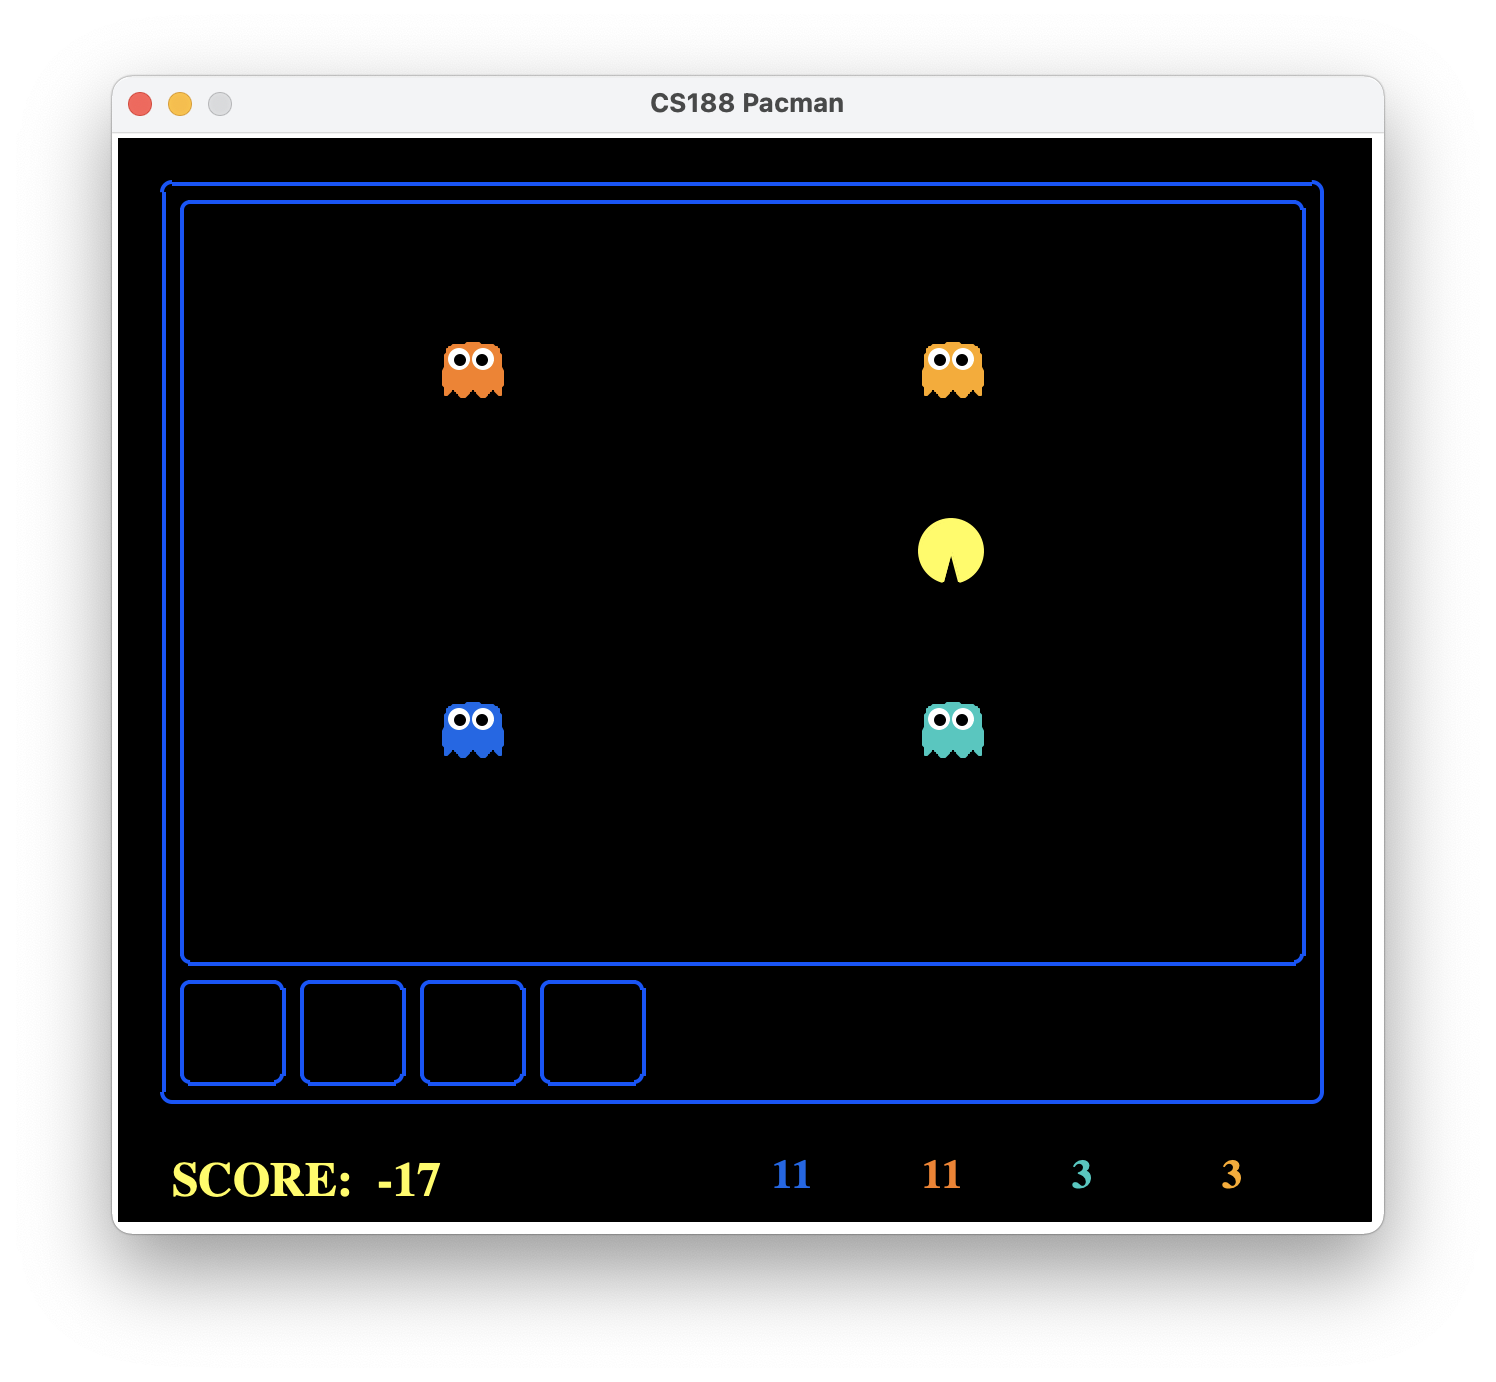
\includegraphics[scale=0.4]{score}
	\vspace*{-7mm}
	\caption{Laberinto \textit{oneHunt}.}
	\label{average_score}
\end{figure}

Durante el proceso para elegir los parámetros \textit{alpha, gamma y epsilon}, los mayoría de los valores de \textit{epsilon} han tomado valores muy próximos a 0, cosa que ha representado una mejora muy significativa en la puntuación obtenida. Esto refleja un comportamiento ya aprendido en la \href{https://poliformat.upv.es/portal/site/ESP_0_2835/tool/c07b745a-0cfd-44f0-a7a2-9bb22f80c3f7?panel=Main}{práctica 1} de la asignatura. En esa práctica aprendimos que si en una estrategia $\epsilon$-greedy el valor de $\epsilon$ es más pequeño, entonces la probabilidad de que un agente tome decisiones aleatorias será menor. Si la aleatoriedad es menor, menor será la inestabilidad del agente, en este caso la del agente Pac-Man. Como consecuencia, el promedio del valor máximo $Q$ será mayor, que es equivalente a una mejor puntuación en el videojuego alcanzando el objetivo del agente. 
\vspace*{2mm}

Los mejores valores encontrados para los parámetros \textit{alpha, gamma y epsilon} son: 0.2, 0.7 y 0.01, respectivamente. A continuación, modificamos su valor en la función \textit{registerInitialState} de la clase \textit{RLAgent} del archivo \textit{bustersAgents.py} de la siguiente manera:
\vspace*{2mm}

\begin{lstlisting}[language=python, basicstyle=\footnotesize]
self.alpha = 0.2
self.gamma = 0.7
self.epsilon = 0.01
\end{lstlisting}

\section{Función de refuerzo}\label{refuerzo}

Una vez que se han adaptado los parámetros del agente Pac-Man ya podemos diseñar la función de refuerzo. La función de refuerzo determinará las recompensas que obtenga el agente. Determinar las recompensas que obtiene el agente con cada acción es clave para su aprendizaje, pues marcará cómo de buenas serán unas acciones frente a otras y por lo tanto determinará qué tipo de comportamientos decidimos potenciar. La siguiente lista enumera las diferentes acciones que he decidido potenciar, con sus valores de recompensa correspondientes:

\begin{itemize}
	\item \textbf{Ganar}. Este estado se muestra cuando el agente Pac-Man gana la partida. Ganamos 1000 puntos de recompensa.
	
	\item \textbf{Comer}. Este estado se muestra cuando el agente Pac-Man se come a un fantasma. Ganamos 100 puntos de recompensa.
	
	\item \textbf{Lejos de un fantasma y lejos de una pared}. Este estado se muestra cuando el agente Pac-Man está al menos a cinco celdas del fantasma más cercano y de la pared más cercana. En este caso, ganamos 1 punto de recompensa.
	
	\item \textbf{Lejos de un fantasma y cerca de una pared}. Este estado se muestra cuando el agente Pac-Man está al menos a cinco celdas del fantasma más cercano y a un máximo de cuatro celdas de la pared más cercana. En este caso, perdemos 1 punto de recompensa.
	
	\item \textbf{Cerca de un fantasma y lejos de una pared} o \textbf{no moverse}. El primer estado (cerca de un fantasma y lejos de una pared) se muestra cuando el agente Pac-Man está a un máximo de cuatro celdas del fantasma más cercano y al menos a cinco celdas de la pared más cercana. El segundo estado (no moverse) se ha añadido porqué en varias de las ejecuciones de prueba, visualmente me fijé que el agente a veces no se movía. Esto provocaba que la partida no pudiera acabar. No llegué a encontrar la solución y añadí este estado aquí, ya que este fenómeno a mi parecer sucedía con más frecuencia cuando el agente se acercaba a un fantasma y se alejaba de una pared. En el caso que el agente no se mueva, perdemos los puntos de recompensa equivalentes a la distancia al fantasma más cercano. Esto también se aplica al primer estado, así que esta situación reveló un caso donde claramente se tendría que mejorar el código de la función de refuerzo, porqué si el agente se encuentra cerca de un fantasma y lejos de una pared, no se tendría que penalizar.
	
	\item \textbf{Cerca de un fantasma y cerca de una pared}. Este estado se muestra cuando el agente Pac-Man está a un máximo de cuatro celdas del fantasma más cercano y de la pared más cercana. En este caso, ganamos 2 puntos de recompensa.
	
	\item \textbf{Cerca de una pared}. Este estado se muestra cuando el agente Pac-Man está a un máximo de cuatro celdas de la pared más cercana. En este caso, perdemos 3 puntos de recompensa.
	
	\item \textbf{Lejos de una pared}. Este estado se muestra cuando el agente Pac-Man está al menos a cinco celdas de la pared más cercana. En este caso, ganamos 1 punto de recompensa.
\end{itemize}

En todas las acciones, el agente Pac-Man recuerda la posición del fantasma más cercano y elegirá una de las direcciones disponibles: \textit{north, east, south o west} para llegar al fantasma por el camino más corto. Como se puede observar, se han definido las recompensas mediante valores enteros, aunque las acciones dependan de la posición de los fantasmas respecto a la posición del agente. Se ha tomado esa decisión al fin de facilitar el código desarrollado y se han definido los valores de recompensa para cada acción en particular. La elección de los valores concretos de recompensa se ha realizado un poco al azar, siguiendo mi propio criterio. La función de refuerzo desarrollada se muestra a continuación:
\vspace*{2mm}

\begin{lstlisting}[caption={Función de refuerzo.}, label={reward}, language=python, basicstyle=\scriptsize]
def getReward(self, state, nextState):
	"""
	Return a reward value based on the information of state and nextState
	"""
	reward = 0
	
	if nextState.isWin():
		return 1000
	
	# distancias al fantasma mas cercano en el siguiente estado
	next_state_ghost_distances = self.getGhostDistances(nextState)
	# distancias al fantasma mas cercano en el estado actual
	actual_state_ghost_distances = self.getGhostDistances(nextState)
	
	# distancia minima al fantasma mas cercano en el siguiente estado
	min_distance_ghost_next_State = min(next_state_ghost_distances, key=lambda t: t[1])[0]
	min_ghost_distance_next_state = nextState.data.ghostDistances[
		min_distance_ghost_next_State]
	# distancia al fantasma mas cercano en el estado actual
	min_distance_ghost_actual_State = min(actual_state_ghost_distances, key=lambda t: t[1])[0]
	min_ghost_distances_actual_state = state.data.ghostDistances[min_distance_ghost_actual_State]
	
	
	# numero de fantasmas en el estado actual
	number_ghost_actual_state = len(list(filter(lambda d: d is not None, 
		state.data.ghostDistances)))
	# numero de fantasmas en el siguiente estado
	number_ghost_next_state = len(list(filter(lambda d: d is not None, 
		nextState.data.ghostDistances)))
	
	# distancia a la pared mas cercana en el estado actual
	actual_state_has_walls = self.directionIsBlocked(state,
	state.getGhostPositions()[min_distance_ghost_next_State])
	# distancia a la pared mas cercana en el siguiente estado
	next_state_has_walls = self.directionIsBlocked(nextState,
	nextState.getGhostPositions()[min_distance_ghost_next_State])
	
	# come fantasma
	if number_ghost_next_state < number_ghost_actual_state:
		reward += 100
	
	# mas lejos de un fantasma y lejos de una pared, no come
	if min_ghost_distance_next_state < min_ghost_distances_actual_state \
			and not actual_state_has_walls \
				and number_ghost_next_state == number_ghost_actual_state:
		reward += 1
	
	# mas lejos de un fantasma y cerca de una pared, no come
	elif min_ghost_distance_next_state < min_ghost_distances_actual_state \
			and actual_state_has_walls \
				and number_ghost_next_state == number_ghost_actual_state:
		reward -= 1
	
	 # mas cerca de un fantasma y lejos de una pared o no come y no se mueve
	elif (min_ghost_distance_next_state > min_ghost_distances_actual_state 
			and not actual_state_has_walls) \
				or (min_ghost_distance_next_state == min_ghost_distances_actual_state
					and number_ghost_next_state == number_ghost_actual_state):
		reward -= min_ghost_distance_next_state
	
	# mas cerca de un fantasma y cerca de una pared, no come
	elif min_ghost_distance_next_state > min_ghost_distances_actual_state \
		and actual_state_has_walls \
			and number_ghost_next_state == number_ghost_actual_state:
		reward += 2
	
	# cerca de una pared, no come
	if not actual_state_has_walls and next_state_has_walls \
			and number_ghost_next_state == number_ghost_actual_state:
		reward -= 3
		
	# lejos de una pared, no come
	elif actual_state_has_walls and not next_state_has_walls \
			and number_ghost_next_state == number_ghost_actual_state:
		reward += 1
	
	return reward
\end{lstlisting}

Los métodos auxiliares de la función de refuerzo como el método \textit{getGhostDistances}, que muestra las distancias entre los fantasmas y el agente Pac-Man (ver Código~\ref{getGhostDistances}), y el método \textit{directionIsBlocked}, que nos indica si la dirección elegida por el agente sería bloqueada por una pared (ver Código~\ref{directionIsBlocked}), se incluyen en la sección~\ref{apendice_reward}.

\section{Código desarrollado}\label{codigo}

Una vez que hemos seleccionado los parámetros que vamos a utilizar para representar cada estado y hemos desarrollado la función de refuerzo que vamos a emplear (ver Código~\ref{reward}), procedemos a la construcción del agente Pac-Man. La implementación del agente consistirá en ir determinando su estado actual en el videojuego. Dado ese estado, se elegirá la acción a dar de acuerdo con los valores de la tabla $Q$. Una vez elegida la acción, se determinará cuál es la dirección más apropiada para la acción dada. A la hora de elegir la siguiente acción, se actualizará el valor $Q$ en la tabla para el estado y la acción anterior, sobre el estado actual obtenido y la mejor acción que devuelve la fórmula expresada en la ecuación~\ref{formula}. Finalmente dado el estado actual del agente, el proceso comenzará de nuevo eligiendo la siguiente acción. Este procedimiento se recoge en la función \textit{update} de la clase \textit{RLAgent} del archivo \textit{bustersAgents.py} (ver Código~\ref{update}), que lleva a cabo el algoritmo \textit{Q-learning}.
\vspace*{3mm}

La fórmula para obtener un nuevo valor $Q$:

\begin{equation}\label{formula}
	Q_{(t+1)}(s_{t},a_{t}) = (1-\alpha) * Q_{t}(s_{t},a_{t}) + \alpha * (R(s_{t},a_{t})) + V_{t}(s_{t+1}) - Q_{t}(s_{t},a_{t})
\end{equation}

donde,

\begin{conditions}
	Q_{(t+1)}(s_{t},a_{t}) & es el nuevo valor $Q$ dado el estado anterior $s_{t}$ y la acción anterior $a_{t}$. \\
	\alpha & es la tasa de aprendizaje. \\
	R(s_{t},a_{t}) & es el valor de recompensa dado el estado anterior $s_{t}$ y la acción anterior $a_{t}$.	\\
	Q_{t}(s_{t},a_{t}) & es el antiguo valor de $Q$ dado el estado anterior $s_{t}$ y la acción anterior $a_{t}$.	\\
	V_{t}(s_{t+1}) & es el valor de aprendizaje dado el nuevo estado $s_{t+1}$.
\end{conditions}
\vspace*{3mm}

La función \textit{update} que lleva a cabo el algoritmo \textit{Q-learning}:
\vspace*{2mm}

\begin{lstlisting}[caption={Función update.}, label={update}, language=python, basicstyle=\footnotesize]
def update(self, state, action, nextState, reward):
	"""
	The parent class calls this to observe a
	state = action => nextState and reward transition.
	You should do your Q-Value update here
	"""	
	print "Started in state:"
	self.printInfo(state)
	print "Took action: ", action
	print "Ended in state:"
	self.printInfo(nextState)
	print "Got reward: ", reward
	print "---------------------------------"

	# buscar el estado actual en la memoria de estados
	state_position = self.computePosition(state)
	action_position = self.actions[action]  # elegir accion
	# actualizar la tabla Q con la accion elegida
	self.q_table[state_position][action_position] = (1 - self.alpha) * 
		self.q_table[state_position][action_position] + self.alpha * (reward + 
			self.gamma * self.getValue(nextState))

	if nextState.isWin():
	# If a terminal state is reached
		self.writeQtable()
\end{lstlisting}

En la función \textit{update} buscamos el estado actual del agente Pac-Man dentro de la memoria de estados con la función \textit{computePosition} (ver Código~\ref{computePosition}), método que se incluye en la sección~\ref{apendice_update}. El agente aprende modificando los valores $Q$ (valores que hay almacenados en la tabla $Q$), de forma que cuando se realiza la acción \textit{action\_position} desde el estado \textit{state\_position}, es el valor $Q$ el que se ve modificado de acuerdo con la fórmula expresada en la ecuación~\ref{formula}. Con la finalidad de que el agente pueda aprender, necesita tener a mano todos los estados que ya haya visitado anteriormente, para poder detectar en cuál de ellos se encuentra a medida que va jugando y, en caso de encontrarse en una situación nueva, registrarla para utilizarla posteriormente. En la implementación de la función \textit{statesMemory}, método que se incluye en la sección~\ref{apendice_update}, estos estados se guardan en forma de lista a medida que se van descubriendo (ver Código~\ref{statesMemory}) y que nombramos memoria de estados.

\begin{figure}[H]
	\begin{minipage}[c]{0.35\linewidth}
		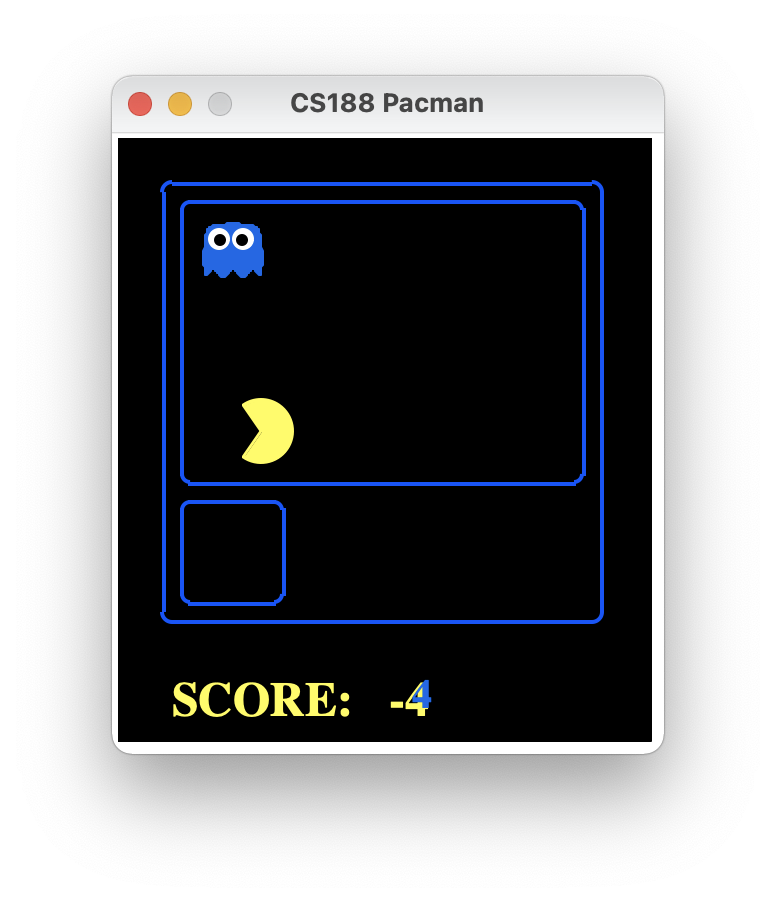
\includegraphics[scale=0.4]{lab1}
		\vspace*{-7mm}
		\caption{Laberinto número uno.}
		\label{lab1}
	\end{minipage}
	\hfill
	\begin{minipage}[c]{0.35\linewidth}
		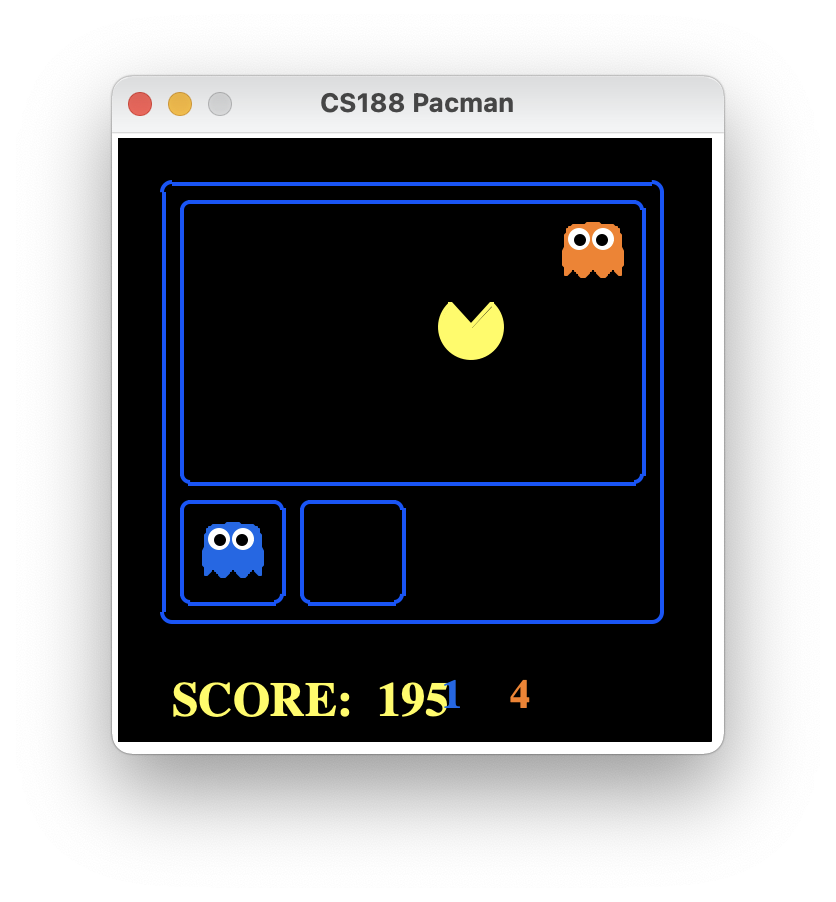
\includegraphics[scale=0.4]{lab2}
		\vspace*{-7mm}
		\caption{Laberinto número dos.}
		\label{lab2}
	\end{minipage}
\end{figure}

\vspace*{-7mm}

\begin{figure}[H]
	\centering
	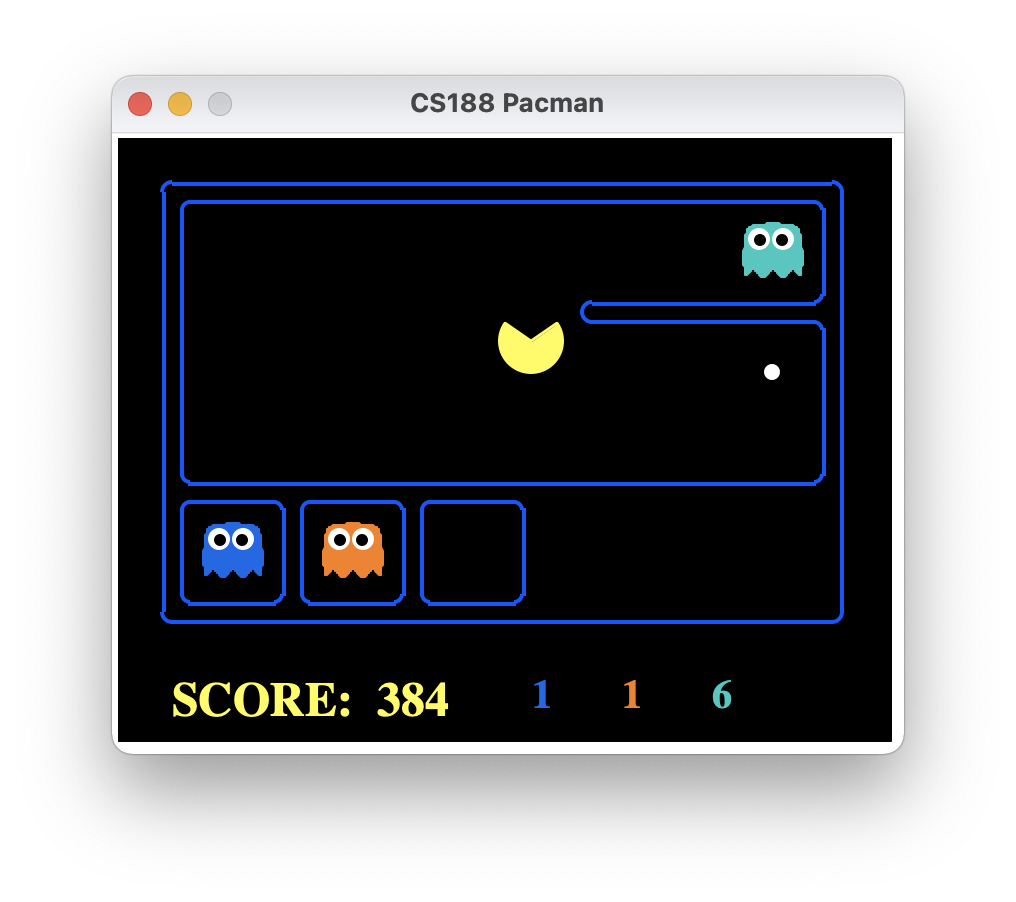
\includegraphics[scale=0.4]{lab3}
	\vspace*{-7mm}
	\caption{Laberinto número tres.}
	\label{lab3}
\end{figure}

Como ya se ha visto en la \href{https://poliformat.upv.es/portal/site/ESP_0_2835/tool/c07b745a-0cfd-44f0-a7a2-9bb22f80c3f7?panel=Main}{práctica 1} de la asignatura, los valores de la tabla $Q$ únicamente son actualizados cuando se cambia de estado, es decir, si al tomar una acción el agente se mantiene en el mismo estado, la tabla $Q$ no se actualiza, sino que la recompensa se acumula de forma que se suman todas las recompensas obtenidas mientras se permanece en un estado, y es cuando se pasa al siguiente estado el momento de modificar la tabla $Q$. 
\vspace*{3mm}

\section{Resultados}\label{resultados}

En esta sección, una vez se ha construido el agente Pac-Man, observaremos su comportamiento en los tres laberintos disponibles. Para empezar, observaremos su comportamiento en el laberinto número uno (ver Figura~\ref{lab1}), ejecutándolo con el siguiente comando:
\vspace*{2mm}

\begin{lstlisting}[language=python, basicstyle=\footnotesize]
python busters.py -p RLAgent -k 1 -l lab1.lay -n 100
\end{lstlisting}

Con este comando ejecutamos durante 100 partidas al agente Pac-Man en el laberinto \textit{lab1}, que únicamente tiene un fantasma (ver Figura~\ref{lab1}). En este punto, me parece importante comentar que en cada ejecución del agente tenemos que inicializar la tabla $Q$ para el algoritmo \textit{Q-learning}. La tabla se puede encontrar en el fichero \textit{qtable.txt}. Si no inicializamos la tabla $Q$, puede que la ejecución del agente no finalice satisfactoriamente. Durante la ejecución del agente en el primer laberinto, veremos que este encontrará rápidamente la mejor solución para resolver el problema a partir de la segunda partida (ver Figura~\ref{result_lab1}), y cada vez veremos que irá más rápido. La puntuación media obtenida (\textit{Average Score}) por el agente es:
\vspace*{2mm}

\begin{figure}[H]
	\centering
	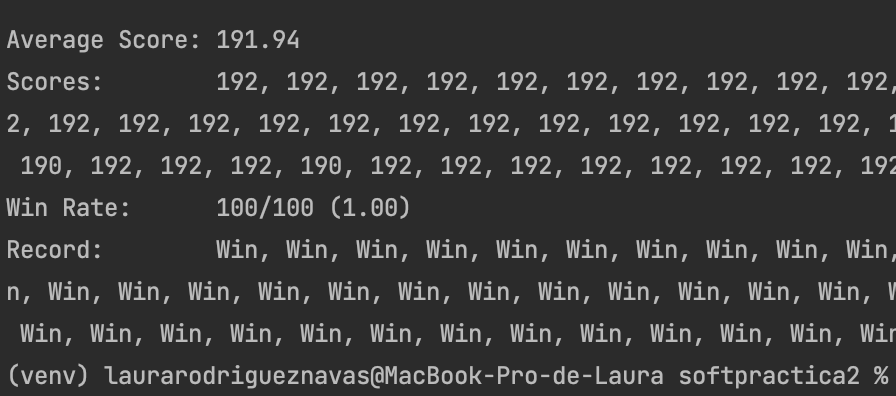
\includegraphics[scale=0.65]{result_lab1}
	\caption{Puntuación obtenida por Pac-Man \\ en el laberinto número uno.}
	\label{result_lab1}
\end{figure}

En esta ejecución, él agente Pac-Man ha ganado en todas las partidas (\textit{Win Rate: 100/100 (1.00)}). La puntuación media obtenida es igual a 191.86 y la mejor puntuación obtenida en una partida es igual a 192. Para ganar una partida obteniendo esta puntuación, donde el fantasma se encuentra en la posición (1,6) y el agente inicialmente en la posición (6,3), el agente debe realizar los 8 movimientos siguientes:
\vspace*{2mm}

\begin{table}[H]
	\centering
	\begin{tabular}{ |c|c|c|c|c| } 
		\hline
		Movimiento & \begin{tabular}[c]{@{}c@{}}Posición\\ de Pac-Man\end{tabular} & \begin{tabular}[c]{@{}c@{}}Dirección\\ de Pac-Man\end{tabular} & Recompensa & Puntuación \\
		\hline
		1 & (6,3) & West & 1 & -1 \\
		2 & (5,3) & West & 1 & -2 \\
		3 & (4,3) & West & 1 & -3 \\
		4 & (3,3) & West & 1 & -4 \\
		5 & (2,3) & West & 1 & -5 \\
		6 & (1,3) & North & 1 & -6 \\
		7 & (1,4) & North & 1 & -7 \\
		8 & (1,5) & North & 100 & -8 \\
		- & (1,6) & - & 1000 & 192 \\
		\hline
	\end{tabular}
	\caption{Movimientos de Pac-Man \\ en el laberinto número uno.}
	\label{movimientos_lab1}
\end{table}

\newpage

Gráficamente:

\begin{table}[H]
	\centering
	\begin{tabular}{ccccccccc}
		&
		0 &
		1 &
		2 &
		3 &
		4 &
		5 &
		6 &
		7 \\ \cline{2-9} 
		\multicolumn{1}{c|}{7} &
		\multicolumn{1}{c|}{\cellcolor[HTML]{000000}} &
		\multicolumn{1}{c|}{\cellcolor[HTML]{000000}} &
		\multicolumn{1}{c|}{\cellcolor[HTML]{000000}} &
		\multicolumn{1}{c|}{\cellcolor[HTML]{000000}} &
		\multicolumn{1}{c|}{\cellcolor[HTML]{000000}} &
		\multicolumn{1}{c|}{\cellcolor[HTML]{000000}} &
		\multicolumn{1}{c|}{\cellcolor[HTML]{000000}} &
		\multicolumn{1}{c|}{\cellcolor[HTML]{000000}} \\ \cline{2-9} 
		\multicolumn{1}{c|}{6} &
		\multicolumn{1}{c|}{\cellcolor[HTML]{000000}} &
		\multicolumn{1}{c|}{G} &
		\multicolumn{1}{c|}{} &
		\multicolumn{1}{c|}{} &
		\multicolumn{1}{c|}{} &
		\multicolumn{1}{c|}{} &
		\multicolumn{1}{c|}{} &
		\multicolumn{1}{c|}{\cellcolor[HTML]{000000}} \\ \cline{2-9} 
		\multicolumn{1}{c|}{5} &
		\multicolumn{1}{c|}{\cellcolor[HTML]{000000}} &
		\multicolumn{1}{c|}{X} &
		\multicolumn{1}{c|}{} &
		\multicolumn{1}{c|}{} &
		\multicolumn{1}{c|}{} &
		\multicolumn{1}{c|}{} &
		\multicolumn{1}{c|}{} &
		\multicolumn{1}{c|}{\cellcolor[HTML]{000000}} \\ \cline{2-9} 
		\multicolumn{1}{c|}{4} &
		\multicolumn{1}{c|}{\cellcolor[HTML]{000000}} &
		\multicolumn{1}{c|}{X} &
		\multicolumn{1}{c|}{} &
		\multicolumn{1}{c|}{} &
		\multicolumn{1}{c|}{} &
		\multicolumn{1}{c|}{} &
		\multicolumn{1}{c|}{} &
		\multicolumn{1}{c|}{\cellcolor[HTML]{000000}} \\ \cline{2-9} 
		\multicolumn{1}{c|}{3} &
		\multicolumn{1}{c|}{\cellcolor[HTML]{000000}} &
		\multicolumn{1}{c|}{X} &
		\multicolumn{1}{c|}{X} &
		\multicolumn{1}{c|}{X} &
		\multicolumn{1}{c|}{X} &
		\multicolumn{1}{c|}{X} &
		\multicolumn{1}{c|}{P} &
		\multicolumn{1}{c|}{\cellcolor[HTML]{000000}} \\ \cline{2-9} 
		\multicolumn{1}{c|}{2} &
		\multicolumn{1}{c|}{\cellcolor[HTML]{000000}} &
		\multicolumn{1}{c|}{} &
		\multicolumn{1}{c|}{} &
		\multicolumn{1}{c|}{} &
		\multicolumn{1}{c|}{} &
		\multicolumn{1}{c|}{} &
		\multicolumn{1}{c|}{} &
		\multicolumn{1}{c|}{\cellcolor[HTML]{000000}} \\ \cline{2-9} 
		\multicolumn{1}{c|}{1} &
		\multicolumn{1}{c|}{\cellcolor[HTML]{000000}} &
		\multicolumn{1}{c|}{} &
		\multicolumn{1}{c|}{} &
		\multicolumn{1}{c|}{} &
		\multicolumn{1}{c|}{} &
		\multicolumn{1}{c|}{} &
		\multicolumn{1}{c|}{} &
		\multicolumn{1}{c|}{\cellcolor[HTML]{000000}} \\ \cline{2-9} 
		\multicolumn{1}{c|}{0} &
		\multicolumn{1}{c|}{\cellcolor[HTML]{000000}} &
		\multicolumn{1}{c|}{\cellcolor[HTML]{000000}} &
		\multicolumn{1}{c|}{\cellcolor[HTML]{000000}} &
		\multicolumn{1}{c|}{\cellcolor[HTML]{000000}} &
		\multicolumn{1}{c|}{\cellcolor[HTML]{000000}} &
		\multicolumn{1}{c|}{\cellcolor[HTML]{000000}} &
		\multicolumn{1}{c|}{\cellcolor[HTML]{000000}} &
		\multicolumn{1}{c|}{\cellcolor[HTML]{000000}} \\ \cline{2-9} 
	\end{tabular}
	\caption{Movimientos de Pac-Man \\ en el laberinto número uno.}
	\label{tabla_lab1}
\end{table}

Volvemos a ejecutar al agente Pac-Man, pero esta vez en el laberinto \textit{lab2}, que tiene dos fantasmas (ver Figura~\ref{lab2}). Para ello ejecutamos el siguiente comando:
\vspace*{2mm}

\begin{lstlisting}[language=python, basicstyle=\footnotesize]
python busters.py -p RLAgent -k 2 -l lab2.lay -n 100
\end{lstlisting}
\vspace*{2mm}

Durante la ejecución del agente Pac-Man en el segundo laberinto, igual que en el primer laberinto, veremos como el agente encontrará rápidamente la mejor solución para resolver el problema a partir de la segunda partida (ver Figura~\ref{result_lab2}). Aunque en este laberinto tardará un poco más que en la ejecución realizada en el primer laberinto, porqué en el segundo laberinto hay dos fantasmas y en el primer laberinto solo uno. En este caso también veremos cómo cada vez irá más rápido. La puntuación media obtenida (\textit{Average Score}) por el agente es:
\vspace*{2mm}

\begin{figure}[H]
	\centering
	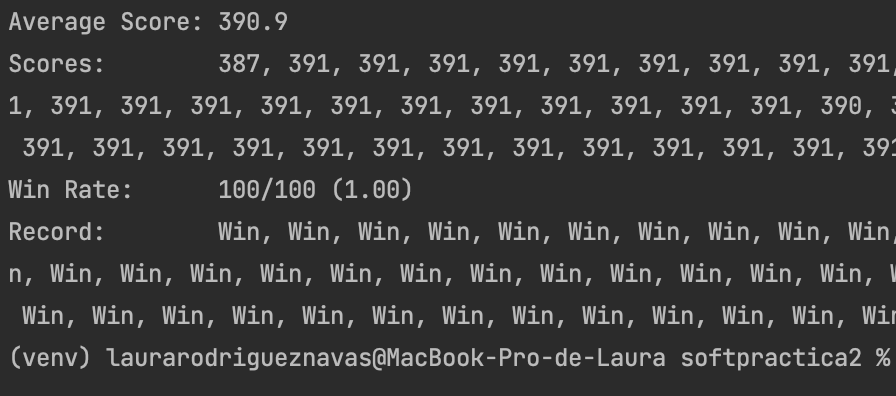
\includegraphics[scale=0.65]{result_lab2}
	\caption{Puntuación obtenida por Pac-Man \\ en el laberinto número dos.}
	\label{result_lab2}
\end{figure}

El agente Pac-Man vuelve a ganar en todas las partidas (\textit{Win Rate: 100/100} (1.00)). La puntuación media obtenida es igual a 390.9. La mejor puntuación obtenida en una partida es igual a 391. En este caso, a diferencia de la ejecución en el primer laberinto, para ganar una partida obteniendo esta puntuación, donde los fantasmas se encuentran en las posiciones (7,6) y (5,4) y el agente inicialmente en la posición (1,3), el agente tiene que realizar 9 movimientos. En la siguiente página se muestran los movimientos.

\begin{table}[H]
	\centering
	\begin{tabular}{ |c|c|c|c|c| } 
		\hline
		Movimiento & \begin{tabular}[c]{@{}c@{}}Posición\\ de Pac-Man\end{tabular} & \begin{tabular}[c]{@{}c@{}}Dirección\\ de Pac-Man\end{tabular} & Recompensa & Puntuación \\
		\hline
		1 & (1,3) & East & 1 & -1 \\
		2 & (2,3) & East & 1 & -2 \\
		3 & (3,3) & East & 1 & -3 \\
		4 & (4,3) & East & 1 & -4 \\
		5 & (5,3) & North & 100 & 195 \\
		6 & (5,4) & East & 1 & 194 \\
		7 & (6,4) & East & 1 & 193 \\
		8 & (7,4) & North & 1 & 192 \\
		9 & (7,5) & North & 100 & 191 \\
		- & (7,6) & - & 1000 & 391 \\
		\hline
	\end{tabular}
	\caption{Movimientos de Pac-Man \\ en el laberinto número dos.}
	\label{movimientos_lab2}
\end{table}
\vspace*{3mm}

Gráficamente:

\begin{table}[H]
	\centering
	\begin{tabular}{cccccccccc}
		&
		0 &
		1 &
		2 &
		3 &
		4 &
		5 &
		6 &
		7 &
		8 \\ \cline{2-9}
		\multicolumn{1}{c|}{7} &
		\multicolumn{1}{c|}{\cellcolor[HTML]{000000}} &
		\multicolumn{1}{c|}{\cellcolor[HTML]{000000}} &
		\multicolumn{1}{c|}{\cellcolor[HTML]{000000}} &
		\multicolumn{1}{c|}{\cellcolor[HTML]{000000}} &
		\multicolumn{1}{c|}{\cellcolor[HTML]{000000}} &
		\multicolumn{1}{c|}{\cellcolor[HTML]{000000}} &
		\multicolumn{1}{c|}{\cellcolor[HTML]{000000}} &
		\multicolumn{1}{c|}{\cellcolor[HTML]{000000}} &
		\cellcolor[HTML]{000000} \\ \cline{2-9}
		\multicolumn{1}{c|}{6} &
		\multicolumn{1}{c|}{\cellcolor[HTML]{000000}} &
		\multicolumn{1}{c|}{} &
		\multicolumn{1}{c|}{} &
		\multicolumn{1}{c|}{} &
		\multicolumn{1}{c|}{} &
		\multicolumn{1}{c|}{} &
		\multicolumn{1}{c|}{} &
		\multicolumn{1}{c|}{G} &
		\cellcolor[HTML]{000000} \\ \cline{2-9}
		\multicolumn{1}{c|}{5} &
		\multicolumn{1}{c|}{\cellcolor[HTML]{000000}} &
		\multicolumn{1}{c|}{} &
		\multicolumn{1}{c|}{} &
		\multicolumn{1}{c|}{} &
		\multicolumn{1}{c|}{} &
		\multicolumn{1}{c|}{} &
		\multicolumn{1}{c|}{} &
		\multicolumn{1}{c|}{X} &
		\cellcolor[HTML]{000000} \\ \cline{2-9}
		\multicolumn{1}{c|}{4} &
		\multicolumn{1}{c|}{\cellcolor[HTML]{000000}} &
		\multicolumn{1}{c|}{} &
		\multicolumn{1}{c|}{} &
		\multicolumn{1}{c|}{} &
		\multicolumn{1}{c|}{} &
		\multicolumn{1}{c|}{G} &
		\multicolumn{1}{c|}{X} &
		\multicolumn{1}{c|}{X} &
		\cellcolor[HTML]{000000} \\ \cline{2-9}
		\multicolumn{1}{c|}{3} &
		\multicolumn{1}{c|}{\cellcolor[HTML]{000000}} &
		\multicolumn{1}{c|}{P} &
		\multicolumn{1}{c|}{X} &
		\multicolumn{1}{c|}{X} &
		\multicolumn{1}{c|}{X} &
		\multicolumn{1}{c|}{X} &
		\multicolumn{1}{c|}{} &
		\multicolumn{1}{c|}{} &
		\cellcolor[HTML]{000000} \\ \cline{2-9}
		\multicolumn{1}{c|}{2} &
		\multicolumn{1}{c|}{\cellcolor[HTML]{000000}} &
		\multicolumn{1}{c|}{} &
		\multicolumn{1}{c|}{} &
		\multicolumn{1}{c|}{} &
		\multicolumn{1}{c|}{} &
		\multicolumn{1}{c|}{} &
		\multicolumn{1}{c|}{} &
		\multicolumn{1}{c|}{} &
		\cellcolor[HTML]{000000} \\ \cline{2-9}
		\multicolumn{1}{c|}{1} &
		\multicolumn{1}{c|}{\cellcolor[HTML]{000000}} &
		\multicolumn{1}{c|}{} &
		\multicolumn{1}{c|}{} &
		\multicolumn{1}{c|}{} &
		\multicolumn{1}{c|}{} &
		\multicolumn{1}{c|}{} &
		\multicolumn{1}{c|}{} &
		\multicolumn{1}{c|}{} &
		\cellcolor[HTML]{000000} \\ \cline{2-9}
		\multicolumn{1}{c|}{0} &
		\multicolumn{1}{c|}{\cellcolor[HTML]{000000}} &
		\multicolumn{1}{c|}{\cellcolor[HTML]{000000}} &
		\multicolumn{1}{c|}{\cellcolor[HTML]{000000}} &
		\multicolumn{1}{c|}{\cellcolor[HTML]{000000}} &
		\multicolumn{1}{c|}{\cellcolor[HTML]{000000}} &
		\multicolumn{1}{c|}{\cellcolor[HTML]{000000}} &
		\multicolumn{1}{c|}{\cellcolor[HTML]{000000}} &
		\multicolumn{1}{c|}{\cellcolor[HTML]{000000}} &
		\cellcolor[HTML]{000000} \\ \cline{2-9}
	\end{tabular}
	\caption{Movimientos de Pac-Man \\ en el laberinto número dos.}
	\label{tabla_lab2}
\end{table}

Finalmente, ejecutamos el agente Pac-Man en el último de los laberintos disponibles, el laberinto \textit{lab3}. Este laberinto tiene 3 fantasmas, una pared interior y una píldora (ver Figura~\ref{lab3}). Para ejecutar el agente usamos el siguiente comando:
\vspace*{2mm}

\begin{lstlisting}[language=python, basicstyle=\footnotesize]
python busters.py -p RLAgent -k 3 -l lab3.lay -n 100
\end{lstlisting}
\vspace*{2mm}

Durante la ejecución del agente Pac-Man en el tercer laberinto, veremos que al agente le costará bastante más trabajo encontrar la mejor solución para resolver el problema. Este comportamiento es normal porqué el laberinto es más grande que los laberintos uno y dos, y además incluye más elementos (tres fantasmas, un muro interior y una píldora). Igualmente, podremos observar como en la mayoría de las veces no encontrará la mejor solución al problema (comer los tres fantasmas y la píldora). En la mayoría de las veces, la mejor solución al problema será que el agente solo se coma a los tres fantasmas. Este comportamiento se puede ver reflejado en la Figura~\ref{result_lab3}. Seguramente este comportamiento se debe a mi implementación de la función de refuerzo. 

\begin{figure}[H]
	\centering
	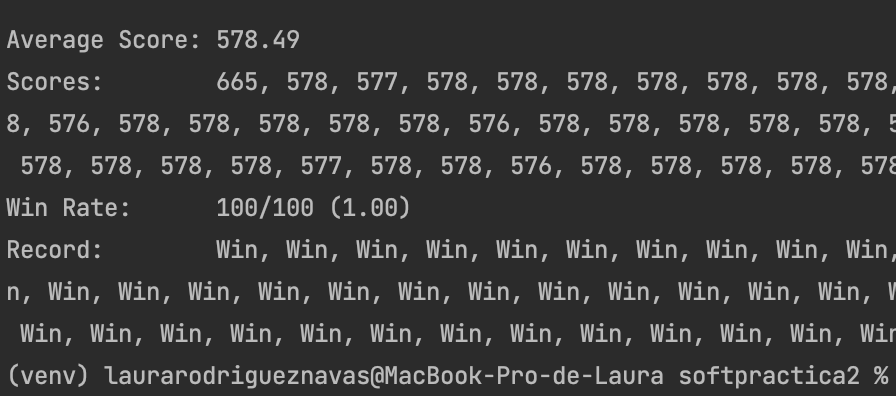
\includegraphics[scale=0.6]{result_lab3}
	\caption{Puntuación obtenida por Pac-Man \\ en el laberinto número tres.}
	\label{result_lab3}
\end{figure}

Aún así, el agente Pac-Man ha ganado en todas las partidas (\textit{Win Rate: 100/100 (1.00)}). La puntuación media obtenida es igual a 613.72. La mejor puntuación obtenida en una partida es igual a 678. En este caso, a diferencia de las ejecuciones en el primer y en el segundo laberinto, para ganar una partida obteniendo esta puntuación, donde los fantasmas se encuentran en las posiciones (10,6), (10,3) y (3,4), la píldora en la posición (10,4) y el agente inicialmente en la posición (1,3), el agente tiene que realizar los 22 movimientos siguientes:
\vspace*{2mm}

\begin{table}[H]
	\centering
	\begin{tabular}{ |c|c|c|c|c| } 
		\hline
		Movimiento & \begin{tabular}[c]{@{}c@{}}Posición\\ de Pac-Man\end{tabular} & \begin{tabular}[c]{@{}c@{}}Dirección\\ de Pac-Man\end{tabular} & Recompensa & Puntuación \\
		\hline
		1 & (1,3) & North & 1 & -1 \\
		2 & (1,4) & East & 1 & -2 \\
		3 & (2,4) & East & 100 & 197 \\
		4 & (3,4) & East & 1 & 196 \\
		5 & (4,4) & East & 1 & 195 \\
		6 & (5,4) & East & 1 & 194 \\
		7 & (6,4) & East & 1 & 193 \\
		8 & (7,4) & East & 1 & 192 \\
		9 & (8,4) & East & 1 & 191 \\
		10 & (9,4) & East & 1 & 290 \\
		11 & (10,4) & South & 100 & 489 \\
		12 & (10,3) & West & 2 & 488 \\
		13 & (9,3) & West & 2 & 487 \\
		14 & (8,3) & West & 2 & 486 \\
		15 & (7,3) & West & 3 & 485 \\
		16 & (6,3) & North & 1 & 484 \\
		17 & (6,4) & North & 1 & 483 \\
		18 & (6,5) & North & 1 & 482 \\
		19 & (6,6) & East & 1 & 481 \\
		20 & (7,6) & East & 1 & 480 \\
		21 & (8,6) & East & 1 & 479 \\
		22 & (9,6) & East & 100 & 578 \\
		- & (10,6) & - & 1000 & 678 \\
		\hline
	\end{tabular}
	\caption{Movimientos de Pac-Man en el laberinto número tres.}
	\label{movimientos_lab3}
\end{table}

Gráficamente:

\begin{table}[H]
	\centering
	\begin{tabular}{ccccccccccccc}
		&
		0 &
		1 &
		2 &
		3 &
		4 &
		5 &
		6 &
		7 &
		8 &
		9 &
		10 &
		11 \\ \cline{2-9}
		\multicolumn{1}{c|}{7} &
		\multicolumn{1}{c|}{\cellcolor[HTML]{000000}} &
		\multicolumn{1}{c|}{\cellcolor[HTML]{000000}} &
		\multicolumn{1}{c|}{\cellcolor[HTML]{000000}} &
		\multicolumn{1}{c|}{\cellcolor[HTML]{000000}} &
		\multicolumn{1}{c|}{\cellcolor[HTML]{000000}} &
		\multicolumn{1}{c|}{\cellcolor[HTML]{000000}} &
		\multicolumn{1}{c|}{\cellcolor[HTML]{000000}} &
		\multicolumn{1}{c|}{\cellcolor[HTML]{000000}} &
		\cellcolor[HTML]{000000} &
		\cellcolor[HTML]{000000} &
		\cellcolor[HTML]{000000} &
		\cellcolor[HTML]{000000} \\ \cline{2-12}
		\multicolumn{1}{c|}{6} &
		\multicolumn{1}{c|}{\cellcolor[HTML]{000000}} &
		\multicolumn{1}{c|}{} &
		\multicolumn{1}{c|}{} &
		\multicolumn{1}{c|}{} &
		\multicolumn{1}{c|}{} &
		\multicolumn{1}{c|}{} &
		\multicolumn{1}{c|}{X} &
		\multicolumn{1}{c|}{X} &
		\multicolumn{1}{c|}{X} &
		\multicolumn{1}{c|}{X} &
		\multicolumn{1}{c|}{G} &
		\cellcolor[HTML]{000000} \\ \cline{2-12}
		\multicolumn{1}{c|}{5} &
		\multicolumn{1}{c|}{\cellcolor[HTML]{000000}} &
		\multicolumn{1}{c|}{} &
		\multicolumn{1}{c|}{} &
		\multicolumn{1}{c|}{} &
		\multicolumn{1}{c|}{} &
		\multicolumn{1}{c|}{} &
		\multicolumn{1}{c|}{X} &
		\multicolumn{1}{c|}{\cellcolor[HTML]{000000}} &
		\multicolumn{1}{c|}{\cellcolor[HTML]{000000}} &
		\multicolumn{1}{c|}{\cellcolor[HTML]{000000}} &
		\multicolumn{1}{c|}{\cellcolor[HTML]{000000}} &
		\cellcolor[HTML]{000000} \\ \cline{2-12}
		\multicolumn{1}{c|}{4} &
		\multicolumn{1}{c|}{\cellcolor[HTML]{000000}} &
		\multicolumn{1}{c|}{X} &
		\multicolumn{1}{c|}{X} &
		\multicolumn{1}{c|}{G} &
		\multicolumn{1}{c|}{X} &
		\multicolumn{1}{c|}{X} &
		\multicolumn{1}{c|}{X} &
		\multicolumn{1}{c|}{X} &
		\multicolumn{1}{c|}{X} &
		\multicolumn{1}{c|}{X} &
		\multicolumn{1}{c|}{$\bullet$} &
		\cellcolor[HTML]{000000} \\ \cline{2-12}
		\multicolumn{1}{c|}{3} &
		\multicolumn{1}{c|}{\cellcolor[HTML]{000000}} &
		\multicolumn{1}{c|}{P} &
		\multicolumn{1}{c|}{} &
		\multicolumn{1}{c|}{} &
		\multicolumn{1}{c|}{} &
		\multicolumn{1}{c|}{} &
		\multicolumn{1}{c|}{X} &
		\multicolumn{1}{c|}{X} &
		\multicolumn{1}{c|}{X} &
		\multicolumn{1}{c|}{X} &
		\multicolumn{1}{c|}{G} &
		\cellcolor[HTML]{000000} \\ \cline{2-12}
		\multicolumn{1}{c|}{2} &
		\multicolumn{1}{c|}{\cellcolor[HTML]{000000}} &
		\multicolumn{1}{c|}{} &
		\multicolumn{1}{c|}{} &
		\multicolumn{1}{c|}{} &
		\multicolumn{1}{c|}{} &
		\multicolumn{1}{c|}{} &
		\multicolumn{1}{c|}{} &
		\multicolumn{1}{c|}{} &
		\multicolumn{1}{c|}{} &
		\multicolumn{1}{c|}{} &
		\multicolumn{1}{c|}{} &
		\cellcolor[HTML]{000000} \\ \cline{2-12}
		\multicolumn{1}{c|}{1} &
		\multicolumn{1}{c|}{\cellcolor[HTML]{000000}} &
		\multicolumn{1}{c|}{} &
		\multicolumn{1}{c|}{} &
		\multicolumn{1}{c|}{} &
		\multicolumn{1}{c|}{} &
		\multicolumn{1}{c|}{} &
		\multicolumn{1}{c|}{} &
		\multicolumn{1}{c|}{} &
		\multicolumn{1}{c|}{} &
		\multicolumn{1}{c|}{} &
		\multicolumn{1}{c|}{} &
		\cellcolor[HTML]{000000} \\ \cline{2-12}
		\multicolumn{1}{c|}{0} &
		\multicolumn{1}{c|}{\cellcolor[HTML]{000000}} &
		\multicolumn{1}{c|}{\cellcolor[HTML]{000000}} &
		\multicolumn{1}{c|}{\cellcolor[HTML]{000000}} &
		\multicolumn{1}{c|}{\cellcolor[HTML]{000000}} &
		\multicolumn{1}{c|}{\cellcolor[HTML]{000000}} &
		\multicolumn{1}{c|}{\cellcolor[HTML]{000000}} &
		\multicolumn{1}{c|}{\cellcolor[HTML]{000000}} &
		\multicolumn{1}{c|}{\cellcolor[HTML]{000000}} &
		\cellcolor[HTML]{000000}{\color[HTML]{333333} } &
		\cellcolor[HTML]{000000}{\color[HTML]{333333} } &
		\cellcolor[HTML]{000000}{\color[HTML]{333333} } &
		\cellcolor[HTML]{000000}{\color[HTML]{333333} } \\ \cline{2-9}
	\end{tabular}
	\caption{Movimientos de Pac-Man \\ en el laberinto número tres.}
	\label{tabla_lab3}
\end{table}

Durante todas las ejecuciones hemos podido observar que el algoritmo \textit{Q-learning} desarrollado en el agente Pac-man es lo suficientemente inteligente para vencer en los tres laberintos disponibles. En cada una de las ejecuciones, el agente Pac-Man ha ido tomando decisiones cada vez que llegaba a una intersección, momento en que miraba el estado actual para ver en qué situación se encontraba, y en base a los conocimientos aprendidos ha tomado la decisión de moverse en una dirección u otra. En aquellos momentos donde también se le ha proporcionado información acerca de los fantasmas, el agente ha tomado decisiones en el momento en que ha percibido a un fantasma demasiado cerca de él, momento en el cual decide atacar, aunque no se encuentre en una intersección. Como no se le ha proporcionado información sobre las píldoras, en el laberinto número tres hemos visto que aparece la aleatoriedad, y según el azar el agente obtendrá una mayor o menor puntuación. Un aspecto a muy importante a mejorar. En resumen, hemos podido comprobar que el agente Pac-Man ha aprendido automáticamente a perseguir a los fantasmas, que son los que le reportan mayor beneficio, eligiendo caminos que contienen la mayor cantidad de fantasmas, desviándose a veces si veía que tenía a un fantasma comestible cerca.

\section{Conclusiones}\label{conclusiones}

En esta práctica se ha aplicado el algoritmo \textit{Q-learning} en su versión determinista para construir un agente Pac-Man que funciona de manera automática y que maximiza la puntuación obtenida en una partida por cada mapa disponible de la práctica: \textit{lab1.lay, lab2.lay y lab3.lay}.  
\vspace*{2mm}

El algoritmo \textit{Q-learning} en este caso, es sin duda un método que parece efectivo. Sin embargo, requiere realizar muchos experimentos para estudiar la viabilidad de las soluciones propuestas. En concreto lo que más problemas me ha causado ha sido la tarea de diseñar los casos, y cómo utilizar la información que contienen estos casos para hacer que el sistema vaya evolucionando a medida que se simulan las partidas en los diferentes laberintos. Conseguir un equilibrio para que los casos no sean demasiado específicos (y por tanto se reutilicen pocas veces), ni tampoco demasiado generales (y no aporten soluciones especialmente útiles), es complicado y requiere de muchas pruebas hasta encontrar los parámetros que mejor se adapten al objetivo perseguido.
\vspace*{2mm}

Los resultados obtenidos por el algoritmo \textit{Q-learning} son mejores de los esperados. Aunque en el tercer laberinto el funcionamiento no es perfecto, la velocidad para encontrar la mejor solución al problema en cada uno de ellos es alta. Seguramente sería muy interesante añadir el comportamiento de diferentes algoritmos estudiados durante la asignatura como \textit{Monte-Carlo} o \textit{SARSA}, y comparar los resultados obtenidos entre ellos.
\vspace*{2mm}

Personalmente uno de los mayores retos de esta práctica ha sido la implementación de todo el código para operar con el agente Pac-Man. El videojuego que se utiliza parece a priori sencillo, pero representa un dominio que se puede volver extremadamente complejo cuando pretendes que un agente aprenda a jugar de manera automática. Como jugadores humanos procesamos información visualmente y la aplicamos muy rápidamente a la toma de decisiones, pero para conseguir que una máquina haga lo mismo, se necesita un alto grado de abstracción de esa información que en ocasiones se ha vuelto un poco difícil de conseguir. En ese momento, ha sido de gran ayuda que el proyecto en el que se basa esta práctica sea tan conocido, ya que muchas personas han tratado de resolver este problema de diferentes maneras, y por la red corren muchos tipos de soluciones que en mi caso me ha dado la posibilidad de aprender y tener una implementación base con la que guiarme.

\section{Apéndice}\label{apendice}

En esta sección se muestran los métodos auxiliares de las funciones \textit{get\_reward} y \textit{update}.

\subsection{Métodos de la función \textit{get\_reward}}\label{apendice_reward}

La función de refuerzo incorpora dos funciones auxiliares que son:

\begin{itemize}
	\item La función \textit{getGhostDistances}, que devuelve las distancias a cada uno de los fantasmas del laberinto en el que se esté ejecutando el agente Pac-Man.
	\item La función \textit{directionIsBlocked}, que devuelve True si la nueva dirección a tomar por el agente Pac-Man será bloqueada por una pared. Devuelve False en caso contrario. También devuelve las distancias a los elementos que bloquean (paredes) y a los elementos que no bloquean (fantasmas).
\end{itemize}

A continuación, observamos su implementación:
\vspace*{3mm}

\begin{lstlisting}[caption={Función getGhostDistances.}, label={getGhostDistances}, language=python, basicstyle=\footnotesize]
def getGhostDistances(gameState):
	"""
	Return distances to each of the ghosts on the map.
	"""
	return [(i, distance) for i, (distance, alive) in enumerate(zip(
		gameState.data.ghostDistances, gameState.getLivingGhosts()[1:])) if alive]
\end{lstlisting}

\begin{lstlisting}[caption={Función directionIsBlocked.}, label={directionIsBlocked}, language=python, basicstyle=\footnotesize]
def directionIsBlocked(gameState, ghost_position):
	"""
	Return True if directions are blocked (walls) and False otherwise (no walls).
	It also returns distances to blocking elements and non-blocking elements.
	"""
	walls = gameState.getWalls()
	walls_array = np.array(walls.data)
	pacman_position = gameState.getPacmanPosition()
	
	x_min = min(pacman_position[0], ghost_position[0])
	x_max = max(pacman_position[0], ghost_position[0]) + 1
	y_min = min(pacman_position[1], ghost_position[1])
	y_max = max(pacman_position[1], ghost_position[1]) + 1
	if y_min < 3:
		y_min = 3
	
	grid_beetween = walls_array[x_min:x_max, y_min:y_max]
	if len(grid_beetween) == 0:
		return False
	
	return np.any(np.all(grid_beetween, axis=1)) or np.any(np.all(grid_beetween, 
		axis=0))
\end{lstlisting}

\subsection{Métodos de la función \textit{update}}\label{apendice_update}

La función \textit{update} también incorpora dos funciones auxiliares que son:

\begin{itemize}
	\item La función \textit{computePosition}, que devuelve la mejor acción dado un estado de la memoria de estados.
	\item La función \textit{statesMemory}, que crea la memoria de estados a medida que el agente Pac-Man se va moviendo en el laberinto en el que se esté ejecutando.
\end{itemize}

A continuación, observamos su implementación:
\vspace*{3mm}

\begin{lstlisting}[caption={Función computePosition.}, label={computePosition}, language=python, basicstyle=\footnotesize]
def computePosition(self, state):
	"""
	Compute the row of the qtable for a given state.
	"""
	pacman_ghost_direction, ghost_position = self.statesMemory(state)
	hasWall = self.directionIsBlocked(state, ghost_position)
	actions_value = 0
	for i, direction in enumerate(pacman_ghost_direction):
		actions_value += min(self.actions[direction], 2) + i * 4
	return int(hasWall) * 8 + actions_value
\end{lstlisting}

\begin{lstlisting}[caption={Función statesMemory.}, label={statesMemory}, language=python, basicstyle=\footnotesize]
def statesMemory(self, gameState):
	"""
	Create states memory.
	"""
	# posicion de pacman
	pacman_position = gameState.getPacmanPosition()
	
	# distancia minima al fantasma mas cercano
	living_ghosts_distances = self.getGhostDistances(gameState)
	min_distance_ghost_index = min(living_ghosts_distances, key=lambda t: t[1])[0]
	
	# posicion del fantasma mas cercano
	nearest_ghost_position = gameState.getGhostPositions()[min_distance_ghost_index]
	
	pacman_ghost_direction = []
	
	if (pacman_position[1] - nearest_ghost_position[1]) != 0 \
			and (pacman_position[1] - nearest_ghost_position[1]) > 0:
		pacman_ghost_direction.append("South")
	if (pacman_position[1] - nearest_ghost_position[1]) != 0 \
			and (pacman_position[1] - nearest_ghost_position[1]) < 0:
		pacman_ghost_direction.append("North")
	if (pacman_position[0] - nearest_ghost_position[0]) != 0 \
			and (pacman_position[0] - nearest_ghost_position[0]) > 0:
		pacman_ghost_direction.append("West")
	if (pacman_position[0] - nearest_ghost_position[0]) != 0 \
			and (pacman_position[0] - nearest_ghost_position[0]) < 0:
		pacman_ghost_direction.append("East")
	
	return pacman_ghost_direction, nearest_ghost_position
\end{lstlisting}

\end{document}
